\section{Geschichte}

\subsection{Grundlagen}
\subsubsection{Theorie}
\settowidth{\MyLenA}{Entscheidbarkeitsprobleme (1931)~~}
\begin{tabular}{@{}p{\the\MyLenA}%
				@{}p{\linewidth-\the\MyLenA}}
	Rechengesetze (15. Jh.) & Adam Ries\\
	Binäre Zahlendarstellung (1703) & Gottfried Leibniz\\
	Boolesche Algebra (1847)	& George Boole\\
	Entscheidbarkeitsprobleme (1931) & Kurt Gödel\\
	Turingmaschine (1936)	& Alan Turing\\
	Von-Neumann-Architektur & John v. Neumann\\
\end{tabular}

\subsubsection{Technik}
\settowidth{\MyLenA}{Programmiersprache Fortran (1955)~~}
\begin{tabular}{@{}p{\the\MyLenA}%
				@{}p{\linewidth-\the\MyLenA}}
	Bipolartransistor (1947) & Bell Laboratories\\
	Programmiersprache Fortran (1955) & IBM\\
	Chomsky-Hierarchie	(1956) & Noam Chomsky\\
	Unix (1969) & Bell Laboratories\\
\end{tabular}

\subsection{Generationen}
\settowidth{\MyLenA}{Generation 5 (seit 1992)~~}
\begin{tabular}{@{}p{\the\MyLenA}%
				@{}p{\linewidth-\the\MyLenA}}
Generation -1 (-1886) & Mechanische Rechmaschinen (Abakus, \dots, Lochkartengesteuerten Zählmaschine)\\
Generation 0 (-1943) & Elektro-mechanische Rechenmaschinen (Z1-Z3)\\
Generation 1 (-1950) & Elektronische Rechner mit Röhren (Eniac, Z4)\\
Generation 2 (-1960) & Elektronische Rechner mit Transistoren (TRADC)\\
Generation 3 (-1968) & Rechner mit integrierten Schaltkreisen (Texas Instruments)\\
Generation 4 (-1984) & Hochintegrierte Computer (IBM-PC, Macintosh)\\
Generation 5 (seit 1992) & Vernetzte und parallele Computer (8 Petaflops mit 80\,000 8-Kern Prozessoren)\\
\end{tabular}

\subsection{Mooresches Gesetz}
\enquote{Die Komplexität integrierter Schaltkreise mit minimalen Komponentenkosten verdoppelt sich regelmässig.}
Etwa alle 20 Monate verdoppelt sich die Anzahl Transistoren pro Fläche. Speicherkarten werden günstiger.

% \subsection{Von-Neumann-Architektur}
% 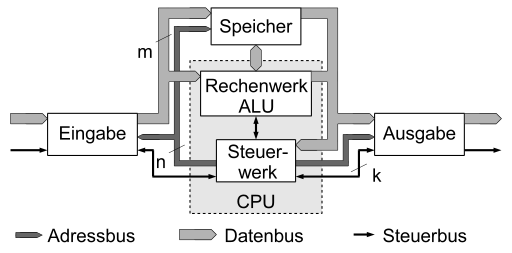
\includegraphics[width=\linewidth]{von_Neumann-_Architektur_de.png}
% \subsubsection{Unterschied zur Harvard-Archiktektur}
% Die Harvard-Architektur trennt zusätzlich den Arbeits- bzw. Datenspeicher physisch vom
% Programmspeicher.

\subsection{Grössenangaben}
\begin{tabular}{c|c|c|c|}
	\textbf{Metrisch} & \textbf{Anzahl} & \textbf{Binärpräfix} & \textbf{Anzahl}\\
	\hline
	Kilobyte [kB] & $10^{3}$ Byte & Kibibyte [KiB] & $2^{10}$ Byte \\
	Megabyte [MB] & $10^{6}$ Byte & Mebibyte [MiB] & $2^{20}$ Byte \\\hline
	Gigabyte [GB] & $10^{9}$ Byte & Gibibyte [GiB] & $2^{30}$ Byte \\
	Terabyte [TB] & $10^{12}$ Byte & Tebibyte [TiB] & $2^{40}$ Byte \\\hline
	Petabyte [PB] & $10^{15}$ Byte & Pebibyte [PiB] & $2^{50}$ Byte \\
	Exabyte [EB] & $10^{18}$ Byte & Exbibyte [EiB] & $2^{60}$ Byte \\\hline
	Zetabyte [ZB] & $10^{21}$ Byte & Zebibyte [ZiB] & $2^{70}$ Byte \\
	Yotabyte [YB] & $10^{24}$ Byte & Yobibyte [YiB] & $2^{80}$ Byte \\
\end{tabular}\\
iB zu B: Exponent = $\log_{2}$ Bytes